% !TEX encoding = IsoLatin
% !TEX TS-program = pdflatex

\documentclass[traditabstract]{aa}
\input Planck.tex

% This is useful to overcome a bug in some versions of
% Adobe Acrobat for Windows
\pdfminorversion=4

\usepackage[breaklinks,colorlinks,citecolor=blue]{hyperref}
\usepackage{amsmath}
\usepackage{natbib}
\usepackage{graphicx}
\usepackage{txfonts}
\usepackage{natbib}

\bibpunct{(}{)}{;}{a}{}{,}

\begin{document}

\title{P00: Planck Paper Plots}

\author{
	Zonca, A. \inst{1}
}

\institute{UCSB\\
	\email{zonca@deepspace.ucsb.edu}
}

\date{\today}

\abstract{Abstract abstract abstract abstract abstract abstract abstract abstract abstract abstract abstract abstract abstract abstract abstract abstract abstract abstract abstract abstract abstract abstract abstract abstract abstract abstract abstract abstract abstract abstract abstract abstract abstract abstract abstract abstract abstract abstract abstract abstract abstract abstract abstract abstract abstract abstract abstract abstract abstract abstract abstract abstract abstract abstract abstract abstract abstract abstract abstract abstract abstract abstract abstract abstract abstract abstract abstract abstract abstract abstract abstract abstract abstract abstract abstract abstract abstract abstract abstract abstract abstract abstract abstract abstract abstract abstract abstract abstract abstract abstract abstract abstract abstract abstract abstract abstract abstract abstract abstract abstract abstract abstract}

\keywords{cosmic microwave background -- Instrumentation: polarimeters -- Methods: data analysis}

\maketitle

\newpage

%%%%%%%%%%%%%%%%%%%%%%%%%%%%%%%%%%%%%%%%%%%%%%%%%%%%%%%%%%%%%%%%%%%%%%

\section{Introduction}

\begin{figure}[h]
\centering
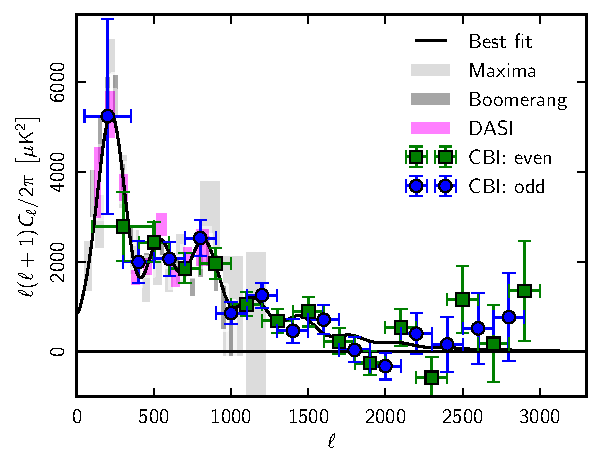
\includegraphics[width=8.8cm]{powerspectrum_88mm.pdf}
\caption{\label{fig:gainCurve} 8.8cm wide} 
\end{figure}

\Planck text text text text text text text text text text text text text text text text text text text text text text text text text text text text text text text text text text text text text text text text text text text text text text text text text text text text text text text text text text text text text text text text text text text text text text text text text text text text text text text text text text text text text text text text text text text text text text text text text text text text text text text text text text text text text text text text text text text text text text text text text text text text text text text text text text text text text text text text text text text text text text text text text text text text text text text text text text text text text text text text text text text text text text text text text text text text text text text text text text text text text text text text text text text text text text text text text text text text text text text text text text text text text text text text text text text text text text text text text text text text text text text text text text text text text text text text text text text text text text text text text text text text text text text text text text text text text text text text text text text text text text text text text text text text text text text text text text text text text text text text text text text text text text text text text text text text text text text text text text text text text 

\Planck text text text text text text text text text text text text text text text text text text text text text text text text text text text text text text text text text text text text text text text text text text text text text text text text text text text text text text text text text text text text text text text text text text text text text text text text text text text text text text text text text text text text text text text text text text text text text text text text text text text text text text text text text text text text text text text text text text text text text text text text text text text text text text text text text text text text text text text text text text text text text text text text text text text text text text text text text text text text text text text text text text text text text text text text text text text text text text text text text text text text text text text text text text text text text text text text text text text text text text text text text text text text text text text text text text text text text text text text text text text text text text text text text text text text text text text text text text text text text text text text text text text text text text text text text text text text text text text text text text text text text text text text text text text text text text text text text text text text text text text text text text text text text text text text text text text text text text text text text text text text text 

\begin{figure*}[h]
\centering
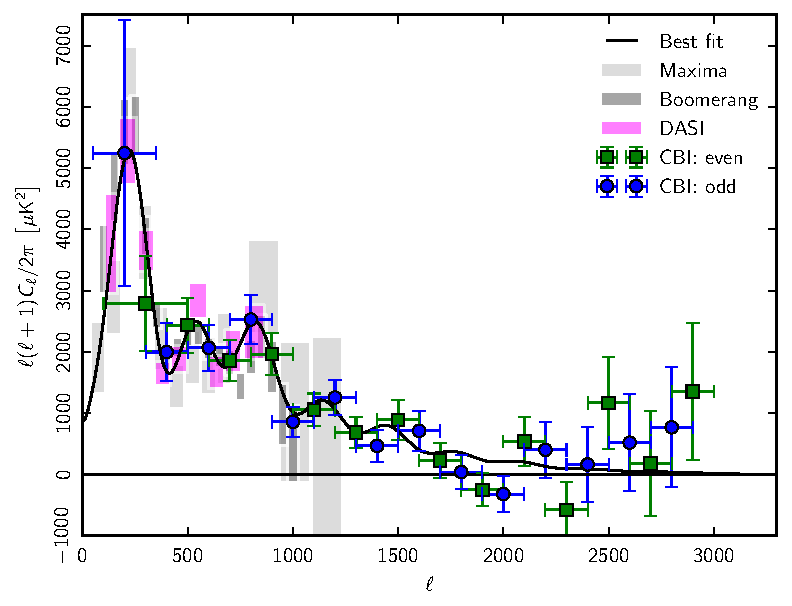
\includegraphics[width=12cm]{powerspectrum_120mm.pdf}
\caption{\label{fig:gainCurve} 12cm wide} 
\end{figure*}

\begin{figure*}[t]
\centering
\includegraphics[width=17cm]{powerspectrum_170mm.pdf}
\caption{\label{fig:gainCurve} Figure created at 17cm wide and setting  width=17cm in includegraphics}
\end{figure*}

\begin{figure*}[t]
\centering
\includegraphics[width=\textwidth]{powerspectrum_170mm.pdf}
\caption{\label{fig:gainCurve} Figure included with width = \ textwidth}
\end{figure*}

\end{document}
